% The Builder tile. Not a screenshot: Builder is a setting rather than a screen,
% and what a reader has to see is that the same three layers are a mould an
% agent fills again for each tool. Drawn like the site's other figures
% (static/blog/tikz/), compiled by `make tiles` to ../builder-setting.svg.
%
% Everything is sized for the tile, which is about 320 px wide on the page: no
% text is smaller than a twentieth of the figure's height, and the words are
% only the five that carry the picture.
\documentclass[tikz,border=0pt]{standalone}
\usetikzlibrary{arrows.meta,positioning,calc}

% the site's palette (static/styles.css)
\definecolor{ink}{HTML}{1B2430}
\definecolor{rule}{HTML}{9AA4AB}
\definecolor{edge}{HTML}{5A646E}
\definecolor{tint}{HTML}{F7E9E9}
\definecolor{red}{HTML}{8B2E2E}
\definecolor{panel}{HTML}{E6EAEC}

% One slab in cabinet projection: #1 x, #2 top y, #3 width, #4 height, #5 fill,
% #6 outline, #7 label. One depth vector throughout, so three stacked slabs read
% as one solid and the small copies read as the same shape made smaller.
\newcommand{\dx}{0.40}
\newcommand{\dy}{0.26}
\newcommand{\slab}[7]{%
  \fill[#5!82!ink] (#1+#3,#2) -- ++(\dx,\dy) -- ++(0,-#4) -- ++(-\dx,-\dy) -- cycle;
  \fill[#5] (#1,#2) -- ++(#3,0) -- ++(\dx,\dy) -- ++(-#3,0) -- cycle;
  \fill[#5] (#1,#2) rectangle ++(#3,-#4);
  \draw[#6] (#1+#3,#2) -- ++(\dx,\dy) -- ++(0,-#4) -- ++(-\dx,-\dy) -- cycle;
  \draw[#6] (#1,#2) -- ++(#3,0) -- ++(\dx,\dy) -- ++(-#3,0) -- cycle;
  \draw[#6] (#1,#2) rectangle ++(#3,-#4);
  \node[font=\sffamily\bfseries\LARGE, text=ink, anchor=west]
       at (#1+0.3,#2-#4/2) {#7};}

% A tool: the same three layers, smaller, named underneath.
\newcommand{\tool}[3]{%
  \slab{#1}{#2}{2.9}{0.52}{white}{draw=rule, line width=0.9pt}{}
  \slab{#1}{#2-0.66}{2.9}{0.38}{tint}{draw=edge, line width=0.9pt, dashed}{}
  \slab{#1}{#2-1.16}{2.9}{0.78}{panel}{draw=ink, line width=1.1pt}{}
  \node[font=\sffamily\large, text=ink, anchor=north west] at (#1,#2-2.12) {#3};}

\begin{document}
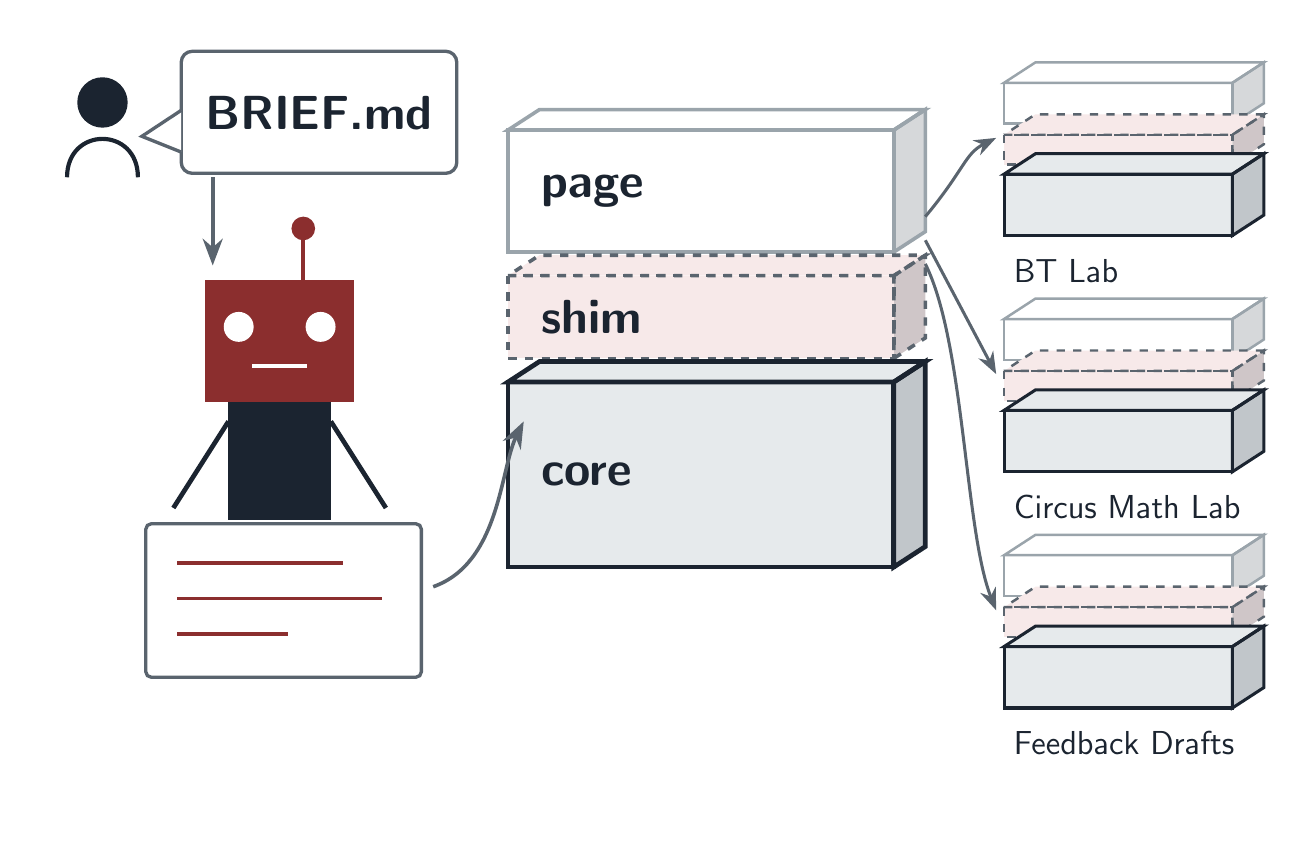
\begin{tikzpicture}[
  font=\sffamily,
  flow/.style={-{Stealth[length=3.4mm]}, draw=edge, line width=1.3pt},
  fan/.style={-{Stealth[length=2.8mm]}, draw=edge, line width=1.1pt}]

\path (0,0) rectangle (16,10);   % 8:5, so the figure fills the tile

% ---- somebody briefs the agent ------------------------------------------
\fill[ink] (0.95,9.05) circle (0.32);
\draw[ink, line width=1.5pt] (0.5,8.1) .. controls (0.5,8.75) and (1.4,8.75) .. (1.4,8.1);
\draw[draw=edge, fill=white, line width=1.2pt, rounded corners=4pt]
      (1.95,8.15) rectangle ++(3.5,1.55);
\fill[white] (1.95,8.95) -- ++(-0.5,-0.33) -- ++(0.5,-0.2) -- cycle;
\draw[edge, line width=1.2pt] (1.95,8.95) -- ++(-0.5,-0.33) -- ++(0.5,-0.2);
\node[font=\sffamily\bfseries\LARGE, text=ink] at (3.7,8.92) {BRIEF.md};

% clear of the aerial, so the brief arrives beside it rather than through it
\draw[flow] (2.35,8.1) -- (2.35,6.98);

% ---- the agent, at work --------------------------------------------------
\fill[red] (2.25,5.25) rectangle ++(1.9,1.55);                % head
\fill[white] (2.68,6.2) circle (0.19);
\fill[white] (3.72,6.2) circle (0.19);
\draw[white, line width=1.3pt] (2.85,5.7) -- ++(0.7,0);       % mouth
\draw[red, line width=1.5pt] (3.5,6.8) -- ++(0,0.55);         % aerial
\fill[red] (3.5,7.45) circle (0.15);
\fill[ink] (2.55,3.75) rectangle ++(1.3,1.5);                 % body, in full view
\draw[ink, line width=1.7pt] (2.55,5.0) -- (1.85,3.9);        % arms down to the keys
\draw[ink, line width=1.7pt] (3.85,5.0) -- (4.55,3.9);
% the thing it is typing on, and three lines of it
\draw[draw=edge, fill=white, line width=1.2pt, rounded corners=2pt]
      (1.5,1.75) rectangle ++(3.5,1.95);
\draw[red, line width=1.3pt] (1.9,3.2) -- ++(2.1,0);
\draw[red, line width=1.3pt] (1.9,2.75) -- ++(2.6,0);
\draw[red, line width=1.3pt] (1.9,2.3) -- ++(1.4,0);

% ---- the setting it builds in: three layers, one solid -------------------
\slab{6.1}{8.7}{4.9}{1.55}{white}{draw=rule, line width=1.3pt}{page}
\slab{6.1}{6.85}{4.9}{1.05}{tint}{draw=edge, line width=1.3pt, dashed}{shim}
\slab{6.1}{5.5}{4.9}{2.35}{panel}{draw=ink, line width=1.7pt}{core}

\draw[flow] (5.15,2.9) .. controls (6.0,3.2) and (6.0,4.4) .. (6.3,5.0);

% ---- the same three layers again, one tool at a time ---------------------
\tool{12.4}{9.3}{BT Lab}
\tool{12.4}{6.3}{Circus Math Lab}
\tool{12.4}{3.3}{Feedback Drafts}

\draw[fan] (11.4,7.6) .. controls (11.9,8.2) and (11.9,8.4) .. (12.3,8.6);
\draw[fan] (11.4,7.3) -- (12.3,5.6);
\draw[fan] (11.4,7.0) .. controls (11.9,6.0) and (11.9,3.6) .. (12.3,2.6);

\end{tikzpicture}
\end{document}
